\documentclass{standalone}

\begin{document}

\section[Dataset]{CHIMeRA datasets}\label{chimera:net}

We have seen how we can extract useful information also from unstructured databases using a web-scraping pipeline.
The \emph{on-line doctor} web pages could be very useful for a toy model application like the \textsf{SymptomsNet} one but if we want produce scientific relevant results we have to take care about the validity of data.
Since the English datasets availability is easier than the Italian one we moved to more \quotes{robust} databases.

As told in the previous sections, there are a lot of studies performed on the disease associations to other biological compounds and in many cases the resulting datasets are public available on Internet.
This is the case of the DisGeNET~\cite{DisGeNet} or DrugBank~\cite{DrugBank} datasets which contain the relationship between a large number of diseases with genes/variants (SNPs) and drugs (and other information), respectively.
The DisGenet \href{https://doi.org/10.1093/nar/gkw943}{web-page} allows to download the datasets already stored into a well structured network format (sparse adjacency matrix, with \numprint{210498} associations between \numprint{117337} SNPs, \numprint{10358} diseases and \numprint{17549} genes) while the DrugBank poses more issues to the treatment of data: the DrugBank database was designed to provide a large set of information related to each drug using its own website and thus it needs a huge pre-processing of the JSON dataset structure to highlight all the possible network associations (\numprint{14812} drugs, \numprint{649} metabolite pathways, \numprint{3256} gene targets, \numprint{40} SNP targets, and \numprint{532} food interactions).
Using the DisGenet we can connect the diseases to their related genes and variants.
From the reviewed format of the DrugBank, instead, we can link each disease to the associated drugs.
Associated to each drug we have also a list of gene and SNP targets which can be merged to the information provided by DisGenet.
Moreover, we can insert also food interactions, metabolite pathways and drug interactions (synergy or not) extracted from DrugBank.
We would stress that, despite the trivial overlaps between the same data sources (genes, diseases and SNPs up to now), just using the rearrangement of these pair of datasets into a network structure, we can already provide a possible extrapolation of the underlying information using the paths between nodes.
Starting from a disease inside the DisGenet, using a single-database approach we can study the \quotes{causality} relationships with the connected genes or SNPs.
Using a multiple-databases (or a network-of-networks structure) approach we can map that disease to other kinds of information like drugs, foods and metabolite pathways.
The aim of such a network-of-networks structure is to unveil relationships hidden by the underwhelming overlap between single-type information across different databases.
The set of different information merged can thus be exploited for applications such as wide-scale drug effect evaluation and design, addressing general diagnostic questions for systems medicine and diseases etiology expansion.
In other words, a network-of-networks structure allows the inference of missing connections using node contraction.
A full list of the information collected by our \textsf{web-scraping} and rearrangement pipelines is shown in Tab.~\ref{tab:chimera_db}.

To enlarge our disease information we looked for other on-line data sources.
A very interesting database is given by HMDB~\cite{HMDB} (\emph{Human Metabolite Data Bank}) which comprises a vast amount of metabolites and metabolite-pathways with the associated drugs and diseases (\numprint{114003} metabolite entries with chemical taxonomies and $\sim$\numprint{25000} human metabolic and disease pathways\footnote{
  The human metabolite-pathways can be divided into different types according to the informations stored in the HMDB dataset.
  The interactions between HMDB and DrugBank was already established through a vast series of hyper-links which connect them using metabolites and metabolite-pathways information.
  In this way we mapped also the information related to the metabolite-pathways types to the DrugBank dataset, obtaining a finer grain nomenclature and classification of these data.
  These informations can be used to improve our disease information.
  In Tab.\ref{tab:chimera_db} is showed only the aggregated data.
}).
The interconnections with the previous discussed datasets are straightforward but in this case the data are not public available and thus we had to apply a \textsf{web-scraping} algorithm to get its information.
An analogous procedure was applied to extract the data included into the \href{https://www.rxlist.com/script/main/hp.asp}{RXList} database.
RXList is an on-line website very similar to the previous discussed auto-diagnosis tools in which we can find associations between diseases and drugs and other several pathogenic associations.
In this case we have a further distinction between diseases: we have diseases related to drugs and diseases connected to other caused-diseases.
We can take care of this kind association using directional links\footnote{
  For sake of clarity, we encountered the same issue also into the DrugBank dataset in which we had intra-drug connections.
}.
We remark that each \textsf{web-scraping} pipeline is customized according to a precise website, so for each analyzed case a different code was developed to address the data extraction.

All these information can enrich our database and the description of a given disease but we have to face on the problem of data merging.
As previously discussed we do not have a unique nomenclature for diseases and thus we can find analogous names (periphrases or synonyms) which identify the same concept (disease).
A useful tool to overcome these issues could be given by a synonym dictionary: a powerful example is given by the CTD~\cite{CTDdb} (\emph{Comparative Toxicogenomics Database}) (\numprint{7212} diseases with mapped synonyms and \numprint{4340} diseases with related phenotypes).
Using the CTD jointly with the SNAP~\cite{biosnapnets} (\emph{Stanford Large Network Dataset Collection}, \numprint{8803} disease terms with related synonyms) database we could enlarge the number of synonyms associated to each disease name.

\begin{table}
\hspace{-2cm}
\begin{tabular}{lcccccccc}
\hline\rowcolor{darkgrayrow}
                        & disease             & drug     & food     & gene     & metabolite & phenotype & SNP      & metabolic \\
\rowcolor{darkgrayrow}
                        &                     &          &          &          &            &           &          & pathway   \\
disease                 & CTD                 & RXList   &    x     & DisGeNET &  HMDB      & CTD       & DisGeNET & HMDB      \\
                        & RXList              &          &          &          &            &           &          &           \\
                        & SNAP                &          &          &          &            &           &          &           \\
drug                    &       RXList        & DrugBank & DrugBank &    x     &    x       &    x      &     x    & DrugBank  \\
food                    &          x          & DrugBank &    x     &    x     &    x       &    x      &     x    &    x      \\
gene                    &      DisGeNET       &    x     &    x     &    x     &    x       &    x      &     x    &    x      \\
metabolite              &       HMDB          &    x     &    x     &    x     &    x       &    x      &     x    & HMDB      \\
phenotype               &        CTD          &    x     &    x     &    x     &    x       &    x      &     x    &    x      \\
SNP                     &      DisGeNET       &    x     &    x     &    x     &    x       &    x      &     x    &    x      \\
metabolic               &        HMDB         & DrugBank &    x     &    x     &  HMDB      &    x      &     x    &    x      \\
pathway                 &                     &          &          &          &            &           &          &           \\
\hline\\
\# nodes                &  63974              & 35161    & 532      & 18799    &  114100    & 13214     & 117337   &  1329     \\
\hline\\
\end{tabular}
\caption{Description of the data mined by the \textsf{CHIMeRA} project before merging.
The datasets were collected using custom web-scraping pipelines and by a rearrangement of the public data.
For each pair of data types we report the list of datasets used to evaluate the interaction.
}
\label{tab:chimera_db}
\end{table}

We remember that the crucial point of our merging procedure is given by the disease nodes since they are the node type shared along (almost) all the databases.
The help given by synonym dictionaries certainly increases the overlap between the mined datasets but we chose to maximize it using a pre-processing NLP pipeline.
So, we started our pipeline using a word \emph{standardization}, i.e converting all the words into their lower case formats and replacing all the punctuation characters with a unique one\footnote{
  An unexpected issue arise in this step: different databases use different enumeration system.
  In some entries we found disease names associated to numbers which identify their multiple types.
  An example could be \quotes{Polyendocrine Autoimmune Syndrome type 1} but at the same time in a second database the same disease could be represented by \quotes{polyendocrine autoimmune TYPE I}.
  Despite the global differences between the two names, given in this case by upper- and lower-cases of some letters and the deletion of some words, a very critical odds is the enumeration style.
  The performances of our pipeline dramatically increased using a \textsf{roman\_number\_converter} algorithm.
}.
Then, we noticed that a not negligible part of words involved into the disease names was useless for the description: words like \quotes{syndrome}, \quotes{disease}, \quotes{disorder}, \quotes{deficiency}, $\cdots$ are not descriptive and so we can filter them.
Now, we could split the disease name into a series of token according to the list of words which compose it (\emph{tokenization}) and sort them.

To further increase the overlap we cut the inflected words to their root form using a \emph{stemming} algorithm: the stemmer strength has to be tuned according to the desired result.
A first processing was performed using a \textsf{Lancaster} stemmer (more aggressive).
If the resulting output was too short to be compared with other names the starting token was processed by a \textsf{Porter Snowball} stemmer (less aggressive).
The stemmer algorithm choice is a very crucial task for NLP because using it we drastically loose information (it is not reversible).
Other processing steps were performed for critical cases encountered during the analyses: these steps constrain our pipeline and they tuned it for the underlying application.

The work-flow outputs include multiple false-positive matches: the pipeline performs a brute force processing and some information lost along the steps could be significants.
In these cases we have multiple processed names belonging to different kind of diseases: an example is shown in Fig.~\ref{fig:chimera_pipe}.
Considering the original name and the processed one (pipeline output) we merged two names using a score match.
This can be achieved introducing the standard word metrics: a common distance between words can be evaluated using the \emph{Levenshtein Distance} which follows the equation

$$
d_{a, b}(i, j) = \left\{ \begin{array}{rc}
  \max(i, j)                                                       & \mbox{if   } \min(i, j) = 0 \\
  \mbox{min} \left\{ \begin{array}{r}
      d_{a, b}(i - 1, j) + 1                     \\
      d_{a, b}(i, j - 1) + 1                     \\
      d_{a, b}(i - 1, j - 1) + 1_{(a \neq b)}    \\
    \end{array}
    \right.                                                        & \mbox{otherwise}            \\

  \end{array}
  \right.
$$
\\
where $a$ and $b$ are two strings of length $|a|$ and $|b|$ respectively.
The \emph{indicator function} $1_{(a \neq b)}$ is equal to $0$ when $a_i = b_j$ and $1$ otherwise.
In this way the Levenshtein distance between $a$ and $b$ can be computed evaluating the distance between the first $i$ characters of $a$ and the first $j$ characters of $b$.
Despite the apparently complex mathematic formulation of this function, the \emph{Levenshtein Distance} is a particular case of the more general \emph{Edit Distance}, i.e a way to quantifying how dissimilar two strings are to one by counting the minimum number of operations required to transform one string into the other.
Also in this case an example could be explainer: given the two string \quotes{\emph{kitten}} and \quotes{\emph{sitting}} their \emph{Levenshtein distance} is equal to 3, in fact

\begin{enumerate}

  \item \textbf{k}itten $\rightarrow$ \textbf{s}itten (substitute \quotes{s} for \quotes{k})
  \item sitt\textbf{e}n $\rightarrow$ sitt\textbf{i}n (substitute \quotes{i} for \quotes{e})
  \item sittin $\rightarrow$ sittin\textbf{g} (insert \quotes{g} at the end)

\end{enumerate}

Using the Levenshtein equation we evaluated the distance between the two original names and we associate the disease to the higher scorer.
A summary scheme of our pipeline is shown in Fig.~\ref{fig:chimera_pipe}.

\begin{figure}[htbp]
\centering
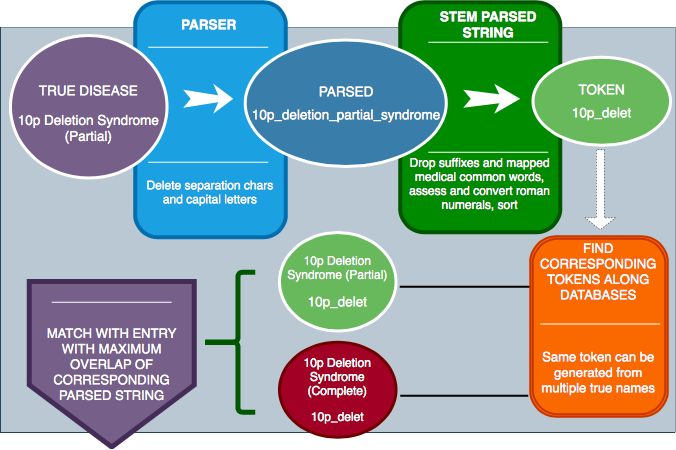
\includegraphics[width=\linewidth]{chimera_pipeline.png}
\caption{Scheme of the NLP pipeline developed in the CHIMeRA project.
The disease words are processed in multiple step as showed in the example.
}
\label{fig:chimera_pipe}
\end{figure}

The described NLP pipeline further increases the overlap between databases (e.g CTD-SNAP 24.17\%; DisGenet-RXList 19.78\%).
We manually supervised and checked the merging procedure taking care to reduce the false positive percentage.
In some cases the overlap percentage remained low also after the application of our pipeline (e.g. RXList-HMDB 8.03\%; SNAP-HMDB 0.39\%).
This behavior could be due to two factors: the first case is related to a deficiency of our pipeline in processing the contained names; in the second case it proved that we were working with complementary databases and thus the real information overlap should be reasonably low.
We took care of these cases and in our checks we always confirmed the second explanation. % riscrivere
This was a very encouraging results since it proved the efficiency of our pipeline and at the same time it confirmed that the union of multiple data sources could effectively enlarge our knowledge.

\begin{figure}[htbp]
\centering
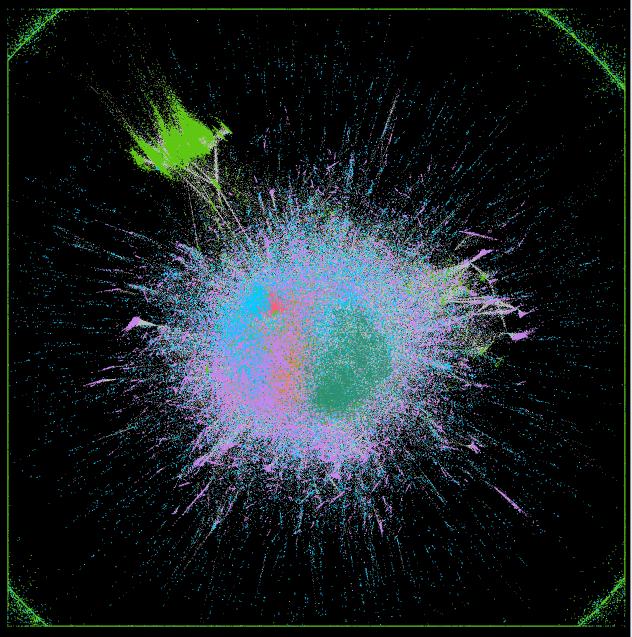
\includegraphics[width=\linewidth]{chimera_plot.png}
\caption{Graphical rendering of the first version of the CHIMeRA network.
The visualization was performed before the inclusion of the DrugBank dataset.
For computational issues we have not performed newer image of the global structure.
In the image we represented disease nodes (azure), gene nodes (orange), SNP nodes (purple), metabolite nodes (light green), drug nodes (pink) and phenotype nodes (dark green).
The visualization was obtained by the \emph{Atlas layout} provided by \textsf{Gephi}.
}
\label{fig:chimera}
\end{figure}

The output of our merging procedure allowed the realization of the \textsf{CHIMeRA} network, i.e a network with more than $3.6\times10^5$ nodes and more than $3.8\times10^7$ links (ref. Fig.\ref{fig:chimera}).
In our resulting structure we have 7 node types: disease (\numprint{63974}), drug (\numprint{35161}), gene (\numprint{18799}), SNP (\numprint{117337}), metabolite (\numprint{114100}), phenotype (\numprint{13214}), metabolite-pathway (\numprint{1329}) and food (532).
The full network adjacency matrix is still a block matrix, i.e we have not all the combinations of information in our databases.
An emblematic case is given by the food nodes: we have food information only into the DrugBank dataset and thus they would be connected only with drug types.
On the other hand our network architecture could be easily improved adding new data sources: the same food nodes are pendant nodes that could be easily connected to other kind of data introducing novel node types or just filling the available blocks.
\textsf{CHIMeRA} is still a work in progress project so we are still looking for improvements and new databases to add.

% disease= 63974
% drug= 35161
% gene= 18799
% SNP= 117337
% metabolite= 114100
% phenotype= 13214
% metapathway= 1329
% food= 532

% total= 364446

\end{document}
